\section{Framework}\label{sec:framework:framework}

This description is for version \versionframe of Framework.\\

\textbf{Remark:}\\
with frame v1.2.3 "Delay Manager" (\texttt{\textquotesingle dm.vhd\textquotesingle }) and "Data Source Multiplexer" (\texttt{\textquotesingle dsmux.vhd\textquotesingle }) are removed because these features were never used in production system, only for tests.
Simmem data not used anymore, because of removed dsmux.
The reason of removing is to get more available resources.\\

Data from the GTH interfaces is demultiplexed (from 240 MHz clock domain to LHC clock domain, see Demux Lane Data \ref{sec:framework:demux_lane_data}) and mapped to objects structure in Lane Mapping Process (LMP) for \ugtl input and SPY I memory.

\subsection{Implementation in firmware}
\label{sec:framework:implementation_firmware}

Listing~\ref{lst:framework:frame_vhd} contains the entity-declaration of \href{\gitbranch/firmware/hdl/payload/frame.vhd}{\texttt{\textquotesingle frame.vhd\textquotesingle }}.\\

\lstinputlisting[label=lst:framework:frame_vhd,language=VHDL,caption=Entity declaration of \texttt{frame.vhd}]{interfaces/frame.vhd}

\clearpage

\medskip
\begin{table}
\footnotesize
\caption{Explanation of Listing~\ref{lst:framework:frame_vhd}}
\vspace{5mm}
\centering
\begin{tabular}{l p{.7\columnwidth}}
\toprule
{Item} & {Explanation}\\
\midrule
\verb|NR_LANES| & number of used optical links.\\
\verb|ipb_clk| & IPBus clock input.\\
\verb|ipb_rst| & IPBus reset input.\\
\verb|ipb_in| & IPBus data input.\\
\verb|ipb_out| & IPBus data output.\\
\verb|ctrs| & TTC control signals input.\\
\verb|clk240| & clock input 240 MHz.\\
\verb|lhc_clk| & clock input (LHC clock).\\
\verb|lhc_rst_o| & reset output.\\
\verb|bc0| & TTC BGo bunch counter reset input.\\
\verb|ec0| & TTC BGo event counter reset input.\\
\verb|oc0| & TTC BGo orbit counter reset input.\\
\verb|start| & TTC BGo start input.\\
\verb|l1a| & L1 access signal input.\\
\verb|bcres_d| & delayed bunch counter reset output.\\
\verb|bcres_d_FDL| & delayed bunch counter reset output fot \ufdl.\\
\verb|start_lumisection| & begin of lumisection output.\\
\verb|lane_data_in| & data from GTHs (optical links) input (240MHz domain).\\
\verb|lane_data_out| & data to GTHs (optical links) output (240MHz domain).\\
\verb|lhc_data_2_gtl_o| & data to \ugtl output (40MHz domain).\\
\verb|prescale_factor_set_in| & prescale factor set data input.\\
\verb|algo_after_gtLogic_rop| & algos after \ugtl input.\\
\verb|algo_after_bxomask_rop| & algos after BX mask input.\\
\verb|algo_after_prescaler_rop| & algos after prescaler input.\\
\verb|local_finor_rop| & local FINOR input.\\
\verb|local_veto_rop| & local VETO input.\\
\verb|finor_rop| & FINOR input.\\
\verb|local_finor_with_veto_2_spy2| & local FINOR with VETO to spy mem input.\\
\bottomrule
\end{tabular}
\label{tab:framework:explanation_frame_vhd}
\end{table}

\clearpage

\subsection{Main parts}

The top-of-hierarchy module of framework (\href{\gitbranch/firmware/hdl/payload/frame.vhd}{\texttt{\textquotesingle frame.vhd\textquotesingle }}) contains
\begin {itemize}
\item demultiplexer of lane data
\item lane mapping
\item spy memories
\item timer counter manager
\item register
\end {itemize}

\subsubsection{Configuration of optical connections} \label{sec:framework:sec_configuration_optical_conn}
The configuration of the optical connections from GMT, Calo-Layer2 and External conditions is done as described in Table~\ref{tab:framework:tab_configuration_optical_conn}, where frame means 32 bits data in a 240 MHz domain.

\begin{table}
\caption{Configuration of optical connections}
\vspace{5mm}
\centering
\begin{tabular}{c|m{.13\columnwidth}|m{.13\columnwidth}|m{.13\columnwidth}|m{.13\columnwidth}|m{.13\columnwidth}|m{.13\columnwidth}|}
\cline{2-7}
 & \multicolumn{6}{c|}{\textbf{frame}} \\\hline
\multicolumn{1}{|c|}{\textbf{link}} & \makebox[.13\columnwidth][c]{\textbf{0}} & \makebox[.13\columnwidth][c]{\textbf{1}} & \makebox[.13\columnwidth][c]{\textbf{2}} & \makebox[.13\columnwidth][c]{\textbf{3}} & \makebox[.13\columnwidth][c]{\textbf{4}} &\makebox[.13\columnwidth][c]{\textbf{5}} \\\hline\hline
\multicolumn{1}{|c|}{0} & reserved & reserved & muon obj. 0 [0..31] & muon obj. 0 [32..63] & muon obj. 1 [0..31] & muon obj. 1 [32..63]\\\hline
\multicolumn{1}{|c|}{1} & reserved & reserved & muon obj. 2 [0..31] & muon obj. 2 [32..63] & muon obj. 3 [0..31] & muon obj. 3 [32..63]\\\hline
\multicolumn{1}{|c|}{2} & reserved & reserved & muon obj. 4 [0..31] & muon obj. 4 [32..63] & muon obj. 5 [0..31] & muon obj. 5 [32..63]\\\hline
\multicolumn{1}{|c|}{3} & reserved & reserved & muon obj. 6 [0..31] & muon obj. 6 [32..63] & muon obj. 7 [0..31] & muon obj. 7 [32..63]\\\hline
\multicolumn{1}{|c|}{4} & \egamma obj. 0 & \egamma obj. 1 & \egamma obj. 2 & \egamma obj. 3 & \egamma obj. 4 & \egamma obj. 5 \\\hline
\multicolumn{1}{|c|}{5} & \egamma obj. 6 & \egamma obj. 7 & \egamma obj. 8 & \egamma obj. 9 & \egamma obj. 10 & \egamma obj. 11 \\\hline
\multicolumn{1}{|c|}{6} & jet obj. 0 & jet obj. 1 & jet obj. 2 & jet obj. 3 & jet obj. 4 & jet obj. 5 \\\hline
\multicolumn{1}{|c|}{7} & jet obj. 6 & jet obj. 7 & jet obj. 8 & jet obj. 9 & jet obj. 10 & jet obj. 11 \\\hline
\multicolumn{1}{|c|}{8} & tau obj. 0 & tau obj. 1 & tau obj. 2 & tau obj. 3 & tau obj. 4 & tau obj. 5 \\\hline
\multicolumn{1}{|c|}{9} & tau obj. 6 & tau obj. 7 & tau obj. 8 & tau obj. 9 & tau obj. 10 & tau obj. 11 \\\hline
\multicolumn{1}{|c|}{\multirow{3}{*}{10}} &
\multicolumn{1}{l|}{\ett} & \htt & \etm & \htm & ET$_{miss}^{HF}$ & HT$_{miss}^{HF}$ \\
\multicolumn{1}{|c|}{} &
\multicolumn{1}{l|}{ETTEM} & TOWER-COUNT & ASYMET & ASYMHT & ASYM-ETHF & ASYM-HTHF \\
\multicolumn{1}{|c|}{} &
\multicolumn{1}{l|}{MBT0HFP} & MBT0HFM & MBT1HFP & MBT1HFM & CENT[3:0] & CENT[7:4] \\\hline
\multicolumn{1}{|c|}{11} & free & free & free & free & free & free \\\hline
\multicolumn{1}{|c|}{12} & external-conditions [0..31] & external-conditions [32..63] & reserved & reserved & reserved & reserved \\\hline
\multicolumn{1}{|c|}{13} & external-conditions [64..95] & external-conditions [96..127] & reserved & reserved & reserved & reserved \\\hline
\multicolumn{1}{|c|}{14} & external-conditions [128..159] & external-conditions [160..191] & reserved & reserved & reserved & reserved \\\hline
\multicolumn{1}{|c|}{15} & external-conditions [192..223] & external-conditions [224..255] & reserved & reserved & reserved & reserved \\\hline
\end{tabular}
\label{tab:framework:tab_configuration_optical_conn}
\end{table}

\clearpage

%------------------------------------------------------------------------------
%
%  Demux Lane data
%
% ------------------------------------------------------------------------------

\subsubsection{Demux Lane Data} \label{sec:framework:demux_lane_data}
Data from GTH interfaces is in the 240 MHz clock domain. The demultiplexing to the LHC clock domain (about 40 MHz) is done in \href{\gitbranch/firmware/hdl/payload/frame/demux_lane_data.vhd}{\texttt{\textquotesingle demux\_lane\_data.vhd\textquotesingle }}, which is instantiated in \href{\gitbranch/firmware/hdl/payload/frame.vhd}{\texttt{\textquotesingle frame.vhd\textquotesingle }} for currently 16 input links.

%------------------------------------------------------------------------------
%
%  Lane Mapping Process
%
% ------------------------------------------------------------------------------

\subsubsection{Lane Mapping Process} \label{sec:framework:lmp}
In the Lane Mapping Process module data from the links are mapped to objects structure defined in \href{\gitbranch/firmware/hdl/packages/lhc_data_pkg.vhd}{\texttt{\textquotesingle lhc\_data\_pkg.vhd\textquotesingle }}.

\paragraph{Implementation}\label{sec:framework:lmp_impl}
Currently lane mapping is "fixed" in \href{\gitbranch/firmware/hdl/payload/frame/lmp.vhd}{\texttt{\textquotesingle lmp.vhd\textquotesingle }} module, see Table \ref{tab:framework:current_lane_mapping} (\esums\textsuperscript{1}: including minimum bias trigger bits, towercounts, asymmetry and centrality bits).

\begin{table}[ht]
\caption{Current lane mapping}
\vspace{5mm}
\centering
\begin{tabular}{|c|l|c|}\hline
\textbf{lane} & \textbf{objects} \\\hline\hline
0 & muon objects 0..1 \\\hline
1 & muon objects 2..3 \\\hline
2 & muon objects 4..5 \\\hline
3 & muon objects 6..7 \\\hline
4 & \egamma objects 0..5 \\\hline
5 & \egamma objects 6..11 \\\hline
6 & jet object 0..5 \\\hline
7 & jet object 6..11 \\\hline
8 & tau object 0..5 \\\hline
9 & tau object 6..11 \\\hline
10 & \esums\footnotemark \\\hline
11 & n/a (currently not used) \\\hline
12 & external-conditions [0..63] \\\hline
13 & external-conditions [64..127] \\\hline
14 & external-conditions [128..191] \\\hline
15 & external-conditions [192..255] \\\hline
\end{tabular}
\label{tab:framework:current_lane_mapping}
\end{table}

\clearpage

%------------------------------------------------------------------------------
%
%  SIM and SPY Memory
%
% ------------------------------------------------------------------------------

\subsubsection{SPY Memory}\label{sec:framework:spy}
\textbf{Remark:}\\
with frame v1.2.3 simulation memory (SIM Memory) data not useable anymore, because of removed "Data Source Multiplexer".
The reason for removing "Data Source Multiplexer" is to get more available resources.\\
SPY memory III for ROP data is not used anymore.\\

Figure \ref{fig_simspy} shows the SPY memory subsystem of Framework.
It is used to calibrate the system and to record results of the \ugtl and \ufdl.

\paragraph{Implementation}\label{sec:framework:spy_impl}
The memory subsystem consists of four three parts, which will be discussed in more detail in the following sections:

\begin{itemize}
\item SPY Trigger
\item SPY Memory I
\item SPY Memory II
\end{itemize}

\begin{figure}[h]
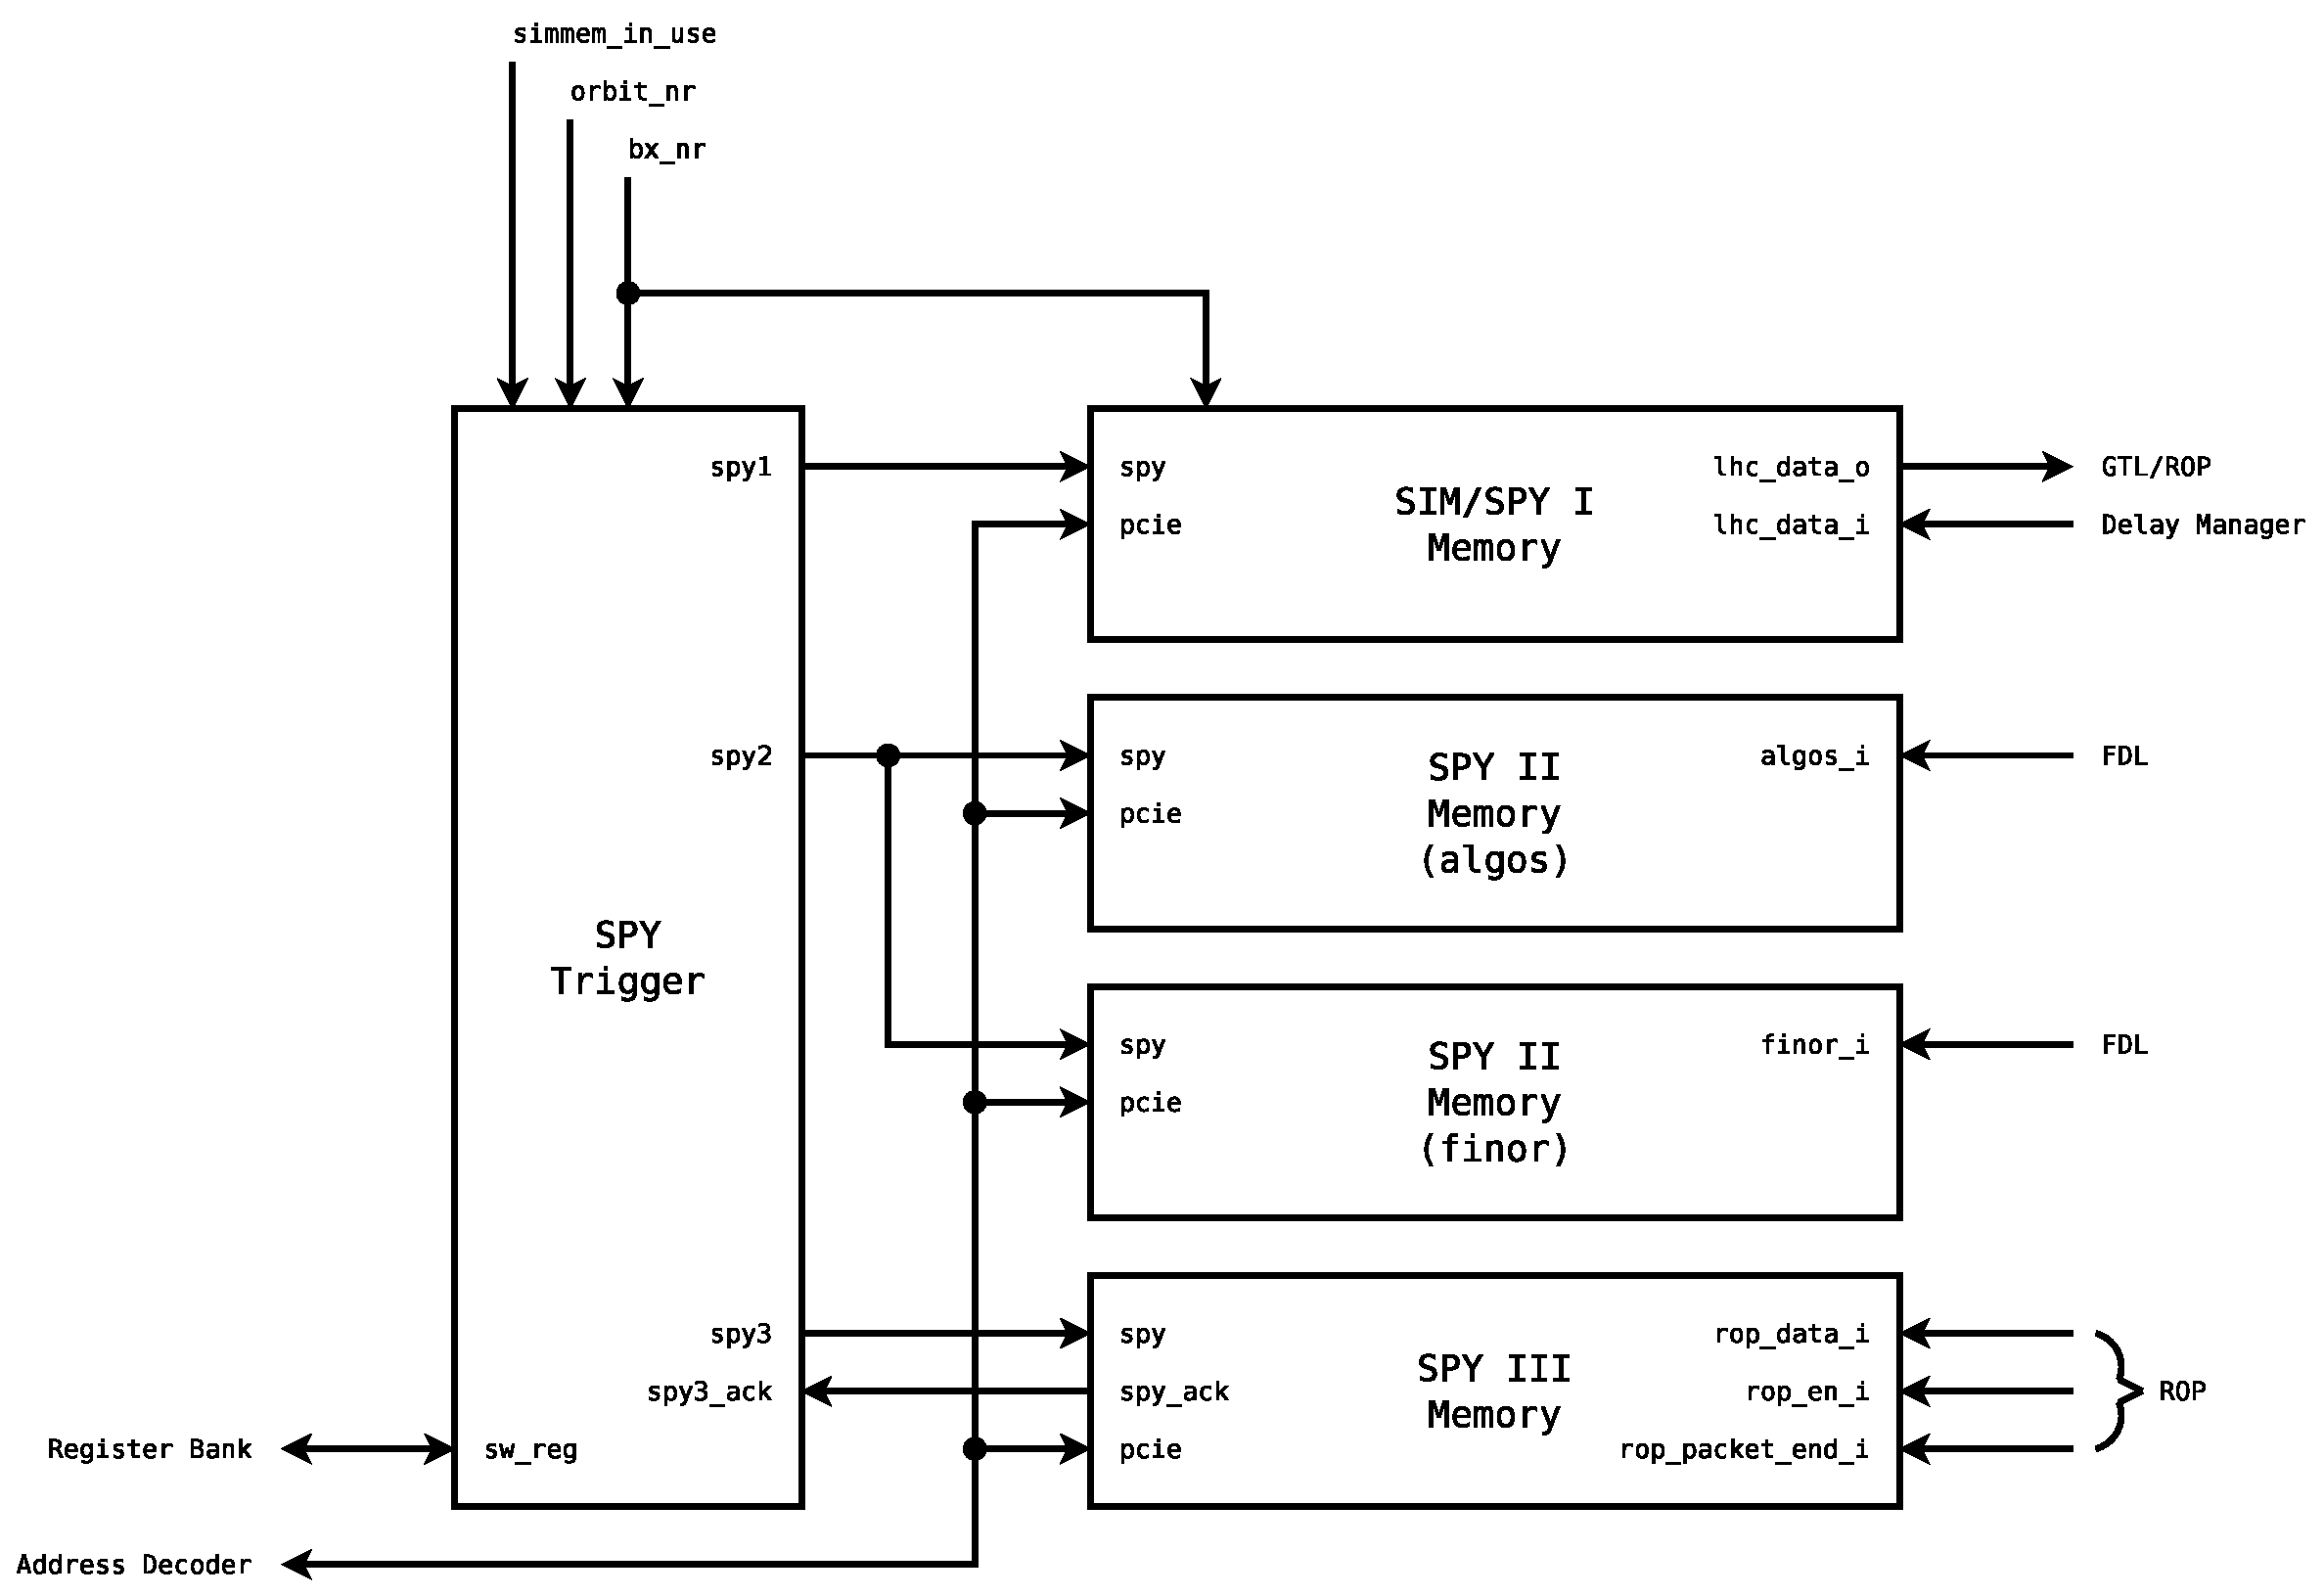
\includegraphics[width=1.0\textwidth]{./figures/simspy}
\caption{Memory subsystem}
\label{fig_simspy}
\end{figure}

\subparagraph{SPY Trigger}\label{sec:framework:spy_trigger}
The SPY trigger controls the SPY memories and decides when data is recorded. It can be configured and controlled using software registers \ref{spy_trig_obrit_nr_reg} and \ref{spy_trig_cfg_reg}.

Listing~\ref{lst:framework:spytrigger_vhd} contains the entity-declaration of the \href{\gitbranch/firmware/hdl/payload/frame/spytrig.vhd}{\texttt{\textquotesingle spytrig.vhd\textquotesingle }}.\\

\lstinputlisting[label=lst:framework:spytrigger_vhd, language=VHDL,caption=SPY trigger interface specification]{interfaces/spytrig.vhd}

When the SPY trigger receives a spy12 command (next or once) over the software register interface it asserts the $spy1$ and $spy2$ signals for the appropriate orbit.
This means that the $spy$ signals go high with the bunch crossing counter reaching the value zero and stay high until it reaches zero again (overflow).

\subparagraph{SPY memory I}
SPY memory I stores data from LMP (coming from GTHs) to check the alignment of the data, for simulation and test purposes. It is composed of 72 4096x32 bits memories (to cover 3564 bunch crossings with 32 bits datawidth) for all input data. The 4096x32 memory has an input port for 32 bits data at the 40MHz clock domain and an IPBus interface to read the content. Memory address is given by bunch crossing counter (40MHz clock domain).

\subparagraph{SPY memory II}
SPY memory II is divided into two subcomponents, to store the $algos$ and $finor$ outputs of the \ufdl, where memory for $algos$ has 16 4096x32 bits memories (16x32=512 algos) and $finor$ is made of only one (for finor with veto). Both have the same architecture as SPY memory I.

%------------------------------------------------------------------------------
%
%  TCM
%
% ------------------------------------------------------------------------------
\subsubsection{Timer Counter Manager}\label{sec:framework:tcm}

The Timer Counter Manager (TCM) provides different counters, listed in Table \ref{tab:framework:tcm_counters} and a set of resisters.

\paragraph{Counter Overview}
\begin{table}[H]
\vspace{5mm}
\begin{scriptsize}
\begin{tabular}{|l|l|l|l|l|}
\hline
\textbf{Counter}    &\textbf{range}     &\textbf{increase condition}      &\textbf{reset condition}  &\textbf{Comments} \\ \hline
bx\_nr (\ref{tcm_bx_nr})             &$0..3563$        &rising\_edge(lhc\_clk)           &overflow                  &             \\ \hline
event\_nr (\ref{tcm_ev_nr})           &$0..2^{32}-1$    &l1a=1 and rising\_edge(lhc\_clk) &BGo: event counter reset &             \\ \hline
trigger\_nr (\ref{tcm_trigger_nr})         &$0..2^{48}-1$    &l1a=1 and rising\_edge(lhc\_clk) &BGo: start run           &             \\ \hline
orbit\_nr (\ref{tcm_orbit_nr})           &$0..2^{48}-1$    &overflow of \textit{bx\_nr}               &BGo: orbit counter reset &             \\ \hline
luminosity\_seg\_nr (\ref{lum_seg_nr}) &$0..2^{32}-1$    &rising\_edge(orbit\_nr(18))      &BGo: orbit counter reset &             \\ \hline
\end{tabular}\caption{Counters of Timer Counter Manager}\label{tab:framework:tcm_counters}
\end{scriptsize}
\end{table}

\paragraph{Counters for bunch crossing-, orbit- and luminosity segment number}
The counter for bunch crossing number (\textit{bx\_nr}) is zero at startup and increased at every LHC clock cycle as depicted in figure \ref{fig:bx_start}. Its maximal value is 3563 (0xdeb), then it automatically overflows and starts at zero again (see figure \ref{fig:bx_normal_operation}). Exactly when \textit{bx\_nr} = 0, delayed BC0 (\textit{bcres\_d}) has to be asserted. Otherwise the counter is out of synchronization. If this happens, the software register \textit{err\_det} is set and the counter waits for the next \textit{bcres\_d} to synchronize again. The value of bunch crossing number can be read from "TCM Bunch Crossing Number Register" (\ref{tcm_bx_nr}).\\
The counter for orbit number (\textit{orbit\_nr}) is 1 at startup and increased at every end of orbit (\textit{bx\_nr} = 3563). It is set to 1 with orbit counter reset (TTC signal oc0). The value of orbit number can be read from "TCM Orbit Number Register" (\ref{tcm_orbit_nr}).\\
The counter for luminosity segment number (\textit{luminosity\_seg\_nr}) is increased, if signal \textit{start} (TTC signal) was applied and counter for orbit number (\textit{orbit\_nr}) is greater than a given value for length of luminosity segment period (currently = 262144 [0x40000], see \href{\gitbranch/firmware/hdl/packages/gt_mp7_core_pkg.vhd}{\texttt{\textquotesingle gt\_mp7\_core\_pkg.vhd\textquotesingle }}). The value of luminosity segmentg number can be read from "TCM Luminosity Segment Number Register" (\ref{lum_seg_nr}).

\begin{figure}[ht]
  \includegraphics[width=1.0\textwidth]{./figures/bx_start}
  \caption{start of the bunch crossing number with the first \textit{bcres\_d}}
  \label{fig:bx_start}
\end{figure}

\begin{figure}[ht]
  \includegraphics[width=1.0\textwidth]{./figures/bx_normal_operation}
  \caption{normal operation of the bunch crossing number}
  \label{fig:bx_normal_operation}
\end{figure}

\paragraph{Bunch crossing counter error}\label{subsec:framework:tcmerrors}
As stated above, \textit{bcres\_d} has to be asserted exactly when \textit{bx\_nr} = 0, otherwise the bunch crossing counter is out of sync. Then the software register \textit{err\_det} is set as depicted in figure \ref{fig:err_det}. Signal \textit{err\_det} can be reset via software event register \textit{err\_det\_reset\_event} as depicted in figure \ref{fig:err_det_reset}.

\begin{figure}[ht]
  \includegraphics[width=1.0\textwidth]{./figures/err_det}
  \caption{set of the software register \textit{err\_det} when \textit{bc\_res\_d} is not asserted correctly}
  \label{fig:err_det}
\end{figure}

\begin{figure}[ht]
  \includegraphics[width=1.0\textwidth]{./figures/err_det_reset}
  \caption{reset of the software register \textit{err\_det} when \textit{err\_det\_reset\_event} toggles}
  \label{fig:err_det_reset}
\end{figure}

The TCM implements two additional counters (\textit{bx\_nr\_chk} and \textit{bx\_nr\_max}) for debugging purposes. These counters are not visible with any other module but readable via software. Counter \textit{bx\_nr\_chk} has 32 bits that increased with every LHC clock cycle and set to 0 with \textit{bcres\_d}. Value \textit{bx\_r\_max} holds the highest \textit{bx\_nr\_chk} ever reached (should be 3563, if the link is aligned).

\paragraph{Counters for event- and trigger number}
The counters for event number (\textit{event\_nr}) and trigger number (\textit{trigger\_nr}) are increased with L1A signal. Event number counter is set to 0 with \textit{ec0} signal, trigger number counter with \textit{start} (TTC signals). The values of event number and trigger number can be read from "TCM Event Number Register" (\ref{tcm_ev_nr}) and "TCM Trigger Number Register" (\ref{tcm_trigger_nr}).

\subsubsection{Software Reset} \label{sec:framework:software_reset}
The software reset module provides the possiblity for a software reset via the software reset register \textit{sw\_reset\_event}, see \ref{tcm_ctrl_reg}.

\subsubsection{Registers}
\label{sec:framework:registers}

\paragraph{Register map}
\label{sec:framework:reg_map}
The register map for Framework has a base address of \verb|0x80000000|.

\begin{longtable}{c p{.25\columnwidth} c p{.45\columnwidth}}
\caption{Framework register map}\\
\hline
Offset & Register name & Access & Description\\
\hline
\hline
\endhead
0x80000000 & \verb|Timestamp| & r & read-only register for timestamp begin of synthesis.\\
0x80000001 & \verb|Hostname| & r & 4 read-only registers for hostname of synthesis platform.\\
0x80000009 & \verb|Username| & r & 4 read-only registers for username of synthesis.\\
0x80000012 & \verb|Frame version| & r & read-only register for Global Trigger firmware version.\\
0x80000013 & \verb|Build version| & r & read-only register for build version of Global Trigger firmware.\\
0x80000800 & \verb|Reset register| & r/w & register for reset pulse and counter reset of counters.\\
0x80200000 & \verb|Spy mem finor| & r/w & 4096 memory addresses for finor and veto.\\
0x80240000 & \verb|Spy mem algos (0)| & r/w & 4096 memory addresses for algos[31:0].\\
0x80241000 & \verb|Spy mem algos (1)| & r/w & 4096 memory addresses for algos[63:32].\\
... & ... & ... & ...\\
0x8024F000 & \verb|Spy mem algos (15)| & r/w & 4096 memory addresses for algos[511:480].\\
0x80300000 & \verb|Spy mem (0)| & r/w & 4096 memory addresses for input data.\\
0x80301000 & \verb|Spy mem (1)| & r/w & 4096 memory addresses for input data.\\
... & ... & ... & ...\\
0x80347000 & \verb|Spy mem (71)| & r/w & 4096 memory addresses for input data.\\
0x80700000 & \vtop{\hbox{\strut \verb|Spytrigger:|}\hbox{\strut \verb|orbit nr low|}} & r/w & register for lower 32 bits of spy trigger orbit number.\\
0x80700001 & \vtop{\hbox{\strut \verb|Spytrigger:|}\hbox{\strut \verb|orbit nr high|}} & r/w & register for higher 32 bits of spy trigger orbit number.\\
0x80700002 & \vtop{\hbox{\strut \verb|Spytrigger:|}\hbox{\strut \verb|control|}} &r/w &  control register for spy12.\\
0x80700003 & \verb|Software reset| & r/w &  software reset register.\\
0x80700010 & \verb|Spytrigger status| & r & status register of spytrigger.\\
0x80700012 & \verb|TCM status| & r & status register of TCM.\\
0x80700016 & \vtop{\hbox{\strut \verb|TCM status:|}\hbox{\strut \verb|orbit nr low|}} & r & read-only register for lower 32 bits of orbit number.\\
0x80700017 & \vtop{\hbox{\strut \verb|TCM status:|}\hbox{\strut \verb|orbit nr high|}} & r & read-only register for higher 32 bits of orbit number.\\
0x80700019 & \vtop{\hbox{\strut \verb|TCM status:|}\hbox{\strut \verb|bx nr max|}} & r & read-only register for maximum Bx number.\\
0x8070001C & \vtop{\hbox{\strut \verb|TCM status:|}\hbox{\strut \verb|lum seg nr|}} & r & read-only register for luminosity segment number.\\
\hline
\label{tab:framework:frame_register_map}
\end{longtable}

\paragraph{Register details}
\label{sec:framework:reg_details}

\begin{register}{htbp}{SPY Trigger Orbit Number Registers}{}
    \label{spy_trig_obrit_nr_reg}
    \regfield{orbit\_nr\_low}{32}{0}{0}%
    \regfield{reserved}{16}{16}{0}%
    \regfield{orbit\_nr\_high}{16}{0}{0}%
    \begin{regdesc}
    \begin{reglist}[Request~Depth]
        \item [orbit\_nr\_low] 32 low bits of the 48 bit orbit number, used for the spy once trigger.
        \item [orbit\_nr\_high] 16 high bits of the 48 bit orbit number, used for the spy once trigger.
    \end{reglist}
    \end{regdesc}
\end{register}

\begin{register}{htbp}{SPY Trigger Configuration Register}{}% name=CONFIG
    \label{spy_trig_cfg_reg}%
    \regfield{spy12\_bsy}{1}{31}{0}%
    \regfield{spy12\_rdy}{1}{29}{0}%
    \regfield{spy12\_err}{1}{27}{0}%
    \regfield{reserved}{21}{6}{0}%
    \regfield{clr\_spy12\_err}{1}{5}{0}%
    \regfield{clr\_spy3\_rdy}{1}{4}{0}%
    \regfield{clr\_spy12\_rdy}{1}{3}{0}%
    \regfield{spy12\_next}{1}{1}{0}%
    \regfield{spy12\_once}{1}{0}{0}%
    \reglabel{Reset}\regnewline%

    \begin{regdesc}
    \begin{reglist}[Request~Depth]
        \item [spy12\_once] Triggers the recording of the selected orbit to SPY memories I and II, when written with 1.
        \item [spy12\_next] Triggers the recording of the next whole orbit to SPY memories I and II, when written with 1.
        \item [clr\_spy12\_rdy] Clears the ready flag of the SPY trigger for SPY memories I and II, when written with 1.
        \item [clr\_spy3\_rdy] Clears the ready flag of the SPY trigger for SPY memory III, when written with 1.
        \item [clr\_spy12\_err] Clears the error flag, when written with 1.
        \item [spy12\_bsy] Indicates that the SPY trigger for SPY memories I and II is busy.
        \item [spy12\_rdy] Indicates that one orbit has been recorded in SPY memories I and II and that the SPY trigger is ready for new commands.
        \item [spy12\_err] Indicates an error condition (Set only when the selected orbit number for the spy once trigger lies in the past and can therefore not be recorded).
    \end{reglist}
    \end{regdesc}
\end{register}

\begin{register}{H}{TCM Bunch Crossing Number Register}{}%
    \label{tcm_bx_nr}
    \regfield{reserved}{20}{12}{0}%
    \regfield{bx\_nr}{12}{0}{0}%
    \begin{regdesc}
    \end{regdesc}
\end{register}

\begin{register}{H}{TCM Event Number Register}{}%
    \label{tcm_ev_nr}
    \regfield{event\_nr}{32}{0}{0}%
    \begin{regdesc}
    \end{regdesc}
\end{register}

\begin{register}{H}{TCM Trigger Number Registers}{}%
    \label{tcm_trigger_nr}
    \regfield{trigger\_nr\_l}{32}{0}{0}%
    \regfield{reserved}{16}{16}{0}%
    \regfield{trigger\_nr\_h}{16}{0}{0}%
    \begin{regdesc}
    \begin{reglist}[Request~Depth]
        \item [trigger\_nr\_l] 32 low bits of the 48 bit trigger number.
        \item [trigger\_nr\_h] 16 high bits of the 48 bit trigger number.
    \end{reglist}
    \end{regdesc}
\end{register}

\begin{register}{H}{TCM Orbit Number Registers}{}%
    \label{tcm_orbit_nr}
    \regfield{orbit\_nr\_l}{32}{0}{0}%
    \regfield{reserved}{16}{16}{0}%
    \regfield{orbit\_nr\_h}{16}{0}{0}%
    \begin{regdesc}
    \begin{reglist}[Request~Depth]
        \item [orbit\_nr\_l] 32 low bits of the 48 bit orbit number.
        \item [orbit\_nr\_h] 16 high bits of the 48 bit orbit number.
    \end{reglist}
    \end{regdesc}
\end{register}

\begin{register}{H}{TCM Luminosity Segment Number Register}{}%
    \label{lum_seg_nr}
    \regfield{luminosity\_seg\_nr}{32}{0}{0}%
    \begin{regdesc}
    \end{regdesc}
\end{register}

\begin{register}{H}{TCM Bunch Crossing Number \ufdl Register}{}%
    \label{tcm_bx_nr_fdl}
    \regfield{reserved}{20}{12}{0}%
    \regfield{bx\_nr\_d\_fdl}{12}{0}{0}%
    \begin{regdesc}
    \end{regdesc}
\end{register}

\begin{register}{H}{TCM Bunch Crossing Number Check Register}{}%
    \label{tcm_bx_nr_chk}
    \regfield{bx\_nr\_chk}{32}{0}{0}%
    \begin{regdesc}
    \end{regdesc}
\end{register}

\begin{register}{H}{TCM Bunch Crossing Number Max Register}{}%
    \label{tcm_bx_nr_max}
    \regfield{bx\_nr\_max}{32}{0}{0}%
    \begin{regdesc}
    \end{regdesc}
\end{register}

\begin{register}{H}{TCM cmd\_ign\_bcres}{}% name=CONFIG
    \label{cmd_ign_bcres}%
    \regfield{reserved}{31}{1}{0}%
    \regfield{cmd\_ign\_bcres}{1}{0}{0}%
    \reglabel{Reset}\regnewline%
    \begin{regdesc}
    \begin{reglist}[Request~Depth]
        \item [cmd\_ign\_bcres] bcres is ignored (not checked) when this is set.
    \end{reglist}
    \end{regdesc}
\end{register}

\begin{register}{H}{TCM err\_det}{}% name=CONFIG
    \label{err_det}%
    \regfield{reserved}{31}{1}{0}%
    \regfield{err\_det}{1}{0}{0}%
    \reglabel{Reset}\regnewline%
    \begin{regdesc}
    \begin{reglist}[Request~Depth]
        \item [err\_det] set when out of synchronization.
    \end{reglist}
    \end{regdesc}
\end{register}

\begin{register}{H}{TCM err\_det\_reset\_event}{}% name=CONFIG
    \label{err_det_reset_event}%
    \regfield{reserved}{31}{1}{0}%
    \regfield{err\_det\_reset\_event}{1}{0}{0}%
    \reglabel{Reset}\regnewline%
    \begin{regdesc}
    \begin{reglist}[Request~Depth]
        \item [err\_det\_reset\_event] resets err\_det.
    \end{reglist}
    \end{regdesc}
\end{register}

\begin{register}{H}{TCM BGo signals}{}% name=CONFIG
    \label{bgos}%
    \regfield{reserved}{31}{4}{0}%
    \regfield{BGo}{4}{0}{0}%
    \reglabel{Reset}\regnewline%
    \begin{regdesc}
    \begin{reglist}[Request~Depth]
        \item [BGo signals] for simulation of BGo signals.
    \end{reglist}
    \end{regdesc}
\end{register}

\begin{register}{H}{TCM BGo\_event}{}% name=CONFIG
    \label{bgos_event}%
    \regfield{reserved}{31}{1}{0}%
    \regfield{BGo\_event}{1}{0}{0}%
    \reglabel{Reset}\regnewline%
    \begin{regdesc}
    \begin{reglist}[Request~Depth]
        \item [BGo\_event] replaces the BGo input signals with the sw-register BGo signals for exactly one clock cycle.
    \end{reglist}
    \end{regdesc}
\end{register}

\begin{register}{H}{TCM luminosity\_seg\_period\_msk}{}% name=CONFIG
    \label{luminosity_seg_period_msk}%
    \regfield{luminosity\_seg\_period\_msk}{32}{0}{0x40000}%
    \reglabel{Reset} %\regnewline%
    \begin{regdesc}
    \begin{reglist}[Request~Depth]
         \item [luminosity\_seg\_period\_msk] luminosity\_seg\_nr is increased when the orbit\_nr mod lum\_seg\_period\_mask = 0.
    \end{reglist}
    \end{regdesc}
\end{register}

\begin{register}{htbp}{Software Reset register}{}% name=CONFIG
    \label{tcm_ctrl_reg}%
    \regfield{reserved}{31}{1}{0}%
    \regfield{sw\_reset\_event}{1}{0}{0}%
    \reglabel{Reset}\regnewline%
    \begin{regdesc}
    \begin{reglist}[Request~Depth]
        \item [sw\_reset\_event] generates a reset signal for exactly one clock cycle.
    \end{reglist}
    \end{regdesc}
\end{register}

\clearpage

